\documentclass[12pt,a4paper]{article}

% ─── Packages ────────────────────────────────────────────────────────────────
\usepackage[margin=1in]{geometry}
\usepackage{amsmath, amssymb}
\usepackage{graphicx}
\usepackage{tikz}
\usetikzlibrary{shapes.geometric, arrows.meta, positioning, fit, backgrounds, calc}
\usepackage{xcolor}
\usepackage{hyperref}
\usepackage{booktabs}
\usepackage{array}
\usepackage{enumitem}
\usepackage{parskip}
\usepackage{fancyhdr}
\setlength{\headheight}{14pt}
\usepackage{titlesec}
\usepackage[hypcap=false]{caption}
\usepackage{mdframed}
\usepackage{multirow}
\usepackage{setspace}

% ─── Colours ─────────────────────────────────────────────────────────────────
\definecolor{primaryblue}{RGB}{108,99,255}
\definecolor{successgreen}{RGB}{16,185,129}
\definecolor{warningyellow}{RGB}{245,158,11}
\definecolor{dangerred}{RGB}{239,68,68}
\definecolor{lightlavender}{RGB}{237,233,254}
\definecolor{slategray}{RGB}{100,116,139}
\definecolor{boxbg}{RGB}{248,250,252}

% ─── Framed box for callouts ──────────────────────────────────────────────────
\newmdenv[
  linecolor=primaryblue!50,
  linewidth=1pt,
  backgroundcolor=lightlavender!40,
  innerleftmargin=12pt,
  innerrightmargin=12pt,
  innertopmargin=8pt,
  innerbottommargin=8pt,
  skipabove=8pt,
  skipbelow=8pt,
]{calloutbox}

\newmdenv[
  linecolor=successgreen!60,
  linewidth=1pt,
  backgroundcolor=successgreen!8,
  innerleftmargin=12pt,
  innerrightmargin=12pt,
  innertopmargin=8pt,
  innerbottommargin=8pt,
  skipabove=8pt,
  skipbelow=8pt,
]{greenbox}

% ─── Section Formatting ───────────────────────────────────────────────────────
\titleformat{\section}
  {\large\bfseries\color{primaryblue}}
  {\thesection.}{0.6em}{}[\titlerule]

\titleformat{\subsection}
  {\normalsize\bfseries\color{slategray}}
  {\thesubsection}{0.5em}{}

\titleformat{\subsubsection}
  {\normalsize\itshape\bfseries}
  {\thesubsubsection}{0.4em}{}

% ─── Header / Footer ─────────────────────────────────────────────────────────
\pagestyle{fancy}
\fancyhf{}
\rhead{\small\color{slategray} Adaptive Learning System Design}
\lhead{\small\color{slategray} ET605 Project}
\rfoot{\small Page \thepage}
\renewcommand{\headrulewidth}{0.4pt}

% ─── TikZ Styles ─────────────────────────────────────────────────────────────
\tikzset{
  block/.style={
    rectangle, rounded corners=5pt,
    minimum width=4.2cm, minimum height=1cm,
    text centered, text width=4cm,
    draw=primaryblue, fill=primaryblue!10,
    font=\small\bfseries
  },
  wideblock/.style={
    rectangle, rounded corners=5pt,
    minimum width=6cm, minimum height=1cm,
    text centered, text width=5.6cm,
    draw=primaryblue, fill=primaryblue!10,
    font=\small\bfseries
  },
  decision/.style={
    diamond, aspect=2.8,
    minimum width=4cm, minimum height=1cm,
    text centered, text width=3.2cm,
    draw=warningyellow!80!black, fill=warningyellow!15,
    font=\small
  },
  terminal/.style={
    rectangle, rounded corners=10pt,
    minimum width=3.8cm, minimum height=1cm,
    text centered, text width=3.2cm,
    draw=successgreen!70!black, fill=successgreen!15,
    font=\small\bfseries
  },
  metricbox/.style={
    rectangle, rounded corners=4pt,
    minimum width=3cm, minimum height=0.8cm,
    text centered, text width=2.8cm,
    draw=slategray!60, fill=boxbg,
    font=\footnotesize
  },
  arrow/.style={-{Stealth[length=6pt]}, thick, color=slategray},
  dasharrow/.style={-{Stealth[length=5pt]}, dashed, thick, color=slategray!60},
}

% ─────────────────────────────────────────────────────────────────────────────
\begin{document}

% ─── Title Page ──────────────────────────────────────────────────────────────
\begin{titlepage}
  \centering
  \vspace*{2cm}

  {\Huge\bfseries\color{primaryblue} Adaptive Learning System Design}\\[0.5cm]
  {\large\color{slategray} AlgebraQuest — Intelligent Tutoring System}\\[0.3cm]
  \rule{\linewidth}{0.8pt}\\[1.5cm]

  {\large\textbf{Course:} ET605 — Learning Engineering \& Technology}\\[0.4cm]
  {\large\textbf{Author:} Chaitanya}\\[0.4cm]
  {\large\textbf{Institution:} Indiana University}\\[0.4cm]
  {\large\textbf{Date:} \today}\\[2cm]

  \begin{mdframed}[linecolor=primaryblue, linewidth=1.2pt,
                   innerleftmargin=14pt, innerrightmargin=14pt,
                   innertopmargin=12pt, innerbottommargin=12pt]
    \centering
    \textit{This document describes the pedagogical design, learning model, and
    adaptive behaviour of an algebra tutoring system. It covers the knowledge
    graph, mastery framework, adaptive difficulty engine, and learning analytics
    system — with a focus on learning science rather than technical
    implementation.}
  \end{mdframed}

  \vfill
  {\small Indiana University Bloomington}
\end{titlepage}

% ─── Table of Contents ───────────────────────────────────────────────────────
\tableofcontents
\newpage

% ─────────────────────────────────────────────────────────────────────────────
\section{System Overview}
% ─────────────────────────────────────────────────────────────────────────────

\subsection{Purpose of the Platform}

AlgebraQuest is a browser-based Intelligent Tutoring System (ITS) designed to
teach foundational algebra concepts to middle-school and early high-school
students. The platform delivers personalised practice sessions in which the
difficulty of questions, the availability of scaffolded hints, and the pacing
of new content all adapt dynamically to the individual learner's demonstrated
competency.

Unlike static worksheets or one-size-fits-all quizzes, AlgebraQuest maintains
a continuous model of each student's knowledge state and updates it after every
answered question. This model drives all subsequent decisions — which question
to present next, whether to offer a hint, and when to unlock new concepts.

\subsection{Why Adaptive Learning?}

A foundational principle of learning science is that instruction is most
effective when it operates in the learner's \emph{zone of proximal
development}: the region between what a learner can do
independently and what they can achieve with appropriate challenge. Systems
that match task difficulty to this zone consistently outperform fixed-difficulty
instruction on retention, transfer, and motivation.

Key benefits of the adaptive approach include:

\begin{itemize}[leftmargin=1.8em]
  \item \textbf{Reduced frustration} — once a concept is mastered, the system
        moves on rather than repeating easy material;
  \item \textbf{Reduced boredom} — difficulty escalates in response to
        demonstrated competency;
  \item \textbf{Targeted remediation} — when specific misconceptions recur, the
        system surfaces corrective instruction before continuing practice;
  \item \textbf{Efficient use of study time} — cognitive effort is concentrated
        on the skills that need it most.
\end{itemize}

\subsection{Knowledge Graph: K01–K15}

The curriculum is modelled as a directed acyclic graph (DAG) of fifteen
\emph{knowledge nodes}, each representing a single teachable concept in
introductory algebra. Prerequisite relationships between nodes define a
partial learning order — a locked node becomes available only after its
prerequisites reach the mastery threshold.

\begin{center}
\begin{tabular}{lll}
  \toprule
  \textbf{Node} & \textbf{Concept Title} & \textbf{Subtopic Area} \\
  \midrule
  K01 & Variables and Constants           & Variables \& Expressions \\
  K02 & Identifying Coefficients          & Variables \& Expressions \\
  K03 & Evaluating Expressions            & Variables \& Expressions \\
  K04 & Writing Expressions from Words    & Variables \& Expressions \\
  K05 & One-Step Addition Equations       & Solving Equations \\
  K06 & One-Step Subtraction Equations    & Solving Equations \\
  K07 & One-Step Multiplication Equations & Solving Equations \\
  K08 & One-Step Division Equations       & Solving Equations \\
  K09 & Recognising Like Terms            & Evaluating \& Simplifying \\
  K10 & Combining Like Terms              & Evaluating \& Simplifying \\
  K11 & Two-Step Equations                & Evaluating \& Simplifying \\
  K12 & Substitution                      & Evaluating \& Simplifying \\
  K13 & Writing Algebraic Expressions     & Variables \& Expressions \\
  K14 & Tables of Values \& Patterns      & Evaluating \& Simplifying \\
  K15 & The Distributive Property         & Simplifying \& Structure \\
  \bottomrule
\end{tabular}
\captionof{table}{Knowledge nodes K01–K15 with concept titles and subtopic areas.}
\end{center}

\bigskip

A representative fragment of the prerequisite chain is shown below.
Arrows indicate that the source node must be mastered before the target
is unlocked.

\begin{center}
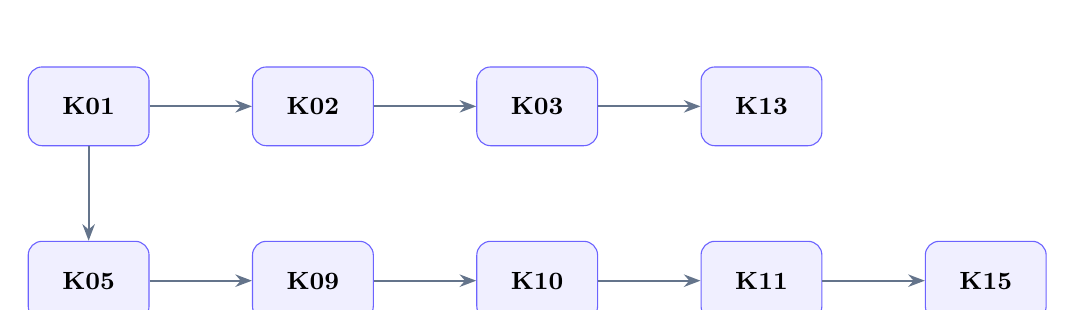
\begin{tikzpicture}[node distance=0.75cm and 1.3cm,
                    every node/.style={font=\small}]
  \node[block, minimum width=1.5cm, text width=1.3cm] (k01) {K01};
  \node[block, minimum width=1.5cm, text width=1.3cm, right=of k01] (k02) {K02};
  \node[block, minimum width=1.5cm, text width=1.3cm, right=of k02] (k03) {K03};
  \node[block, minimum width=1.5cm, text width=1.3cm, right=of k03] (k13) {K13};

  \node[block, minimum width=1.5cm, text width=1.3cm, below=1.2cm of k01] (k05) {K05};
  \node[block, minimum width=1.5cm, text width=1.3cm, right=of k05] (k09) {K09};
  \node[block, minimum width=1.5cm, text width=1.3cm, right=of k09] (k10) {K10};
  \node[block, minimum width=1.5cm, text width=1.3cm, right=of k10] (k11) {K11};
  \node[block, minimum width=1.5cm, text width=1.3cm, right=of k11] (k15) {K15};

  \draw[arrow] (k01) -- (k02);
  \draw[arrow] (k02) -- (k03);
  \draw[arrow] (k03) -- (k13);
  \draw[arrow] (k01) -- (k05);
  \draw[arrow] (k05) -- (k09);
  \draw[arrow] (k09) -- (k10);
  \draw[arrow] (k10) -- (k11);
  \draw[arrow] (k11) -- (k15);
\end{tikzpicture}
\end{center}

% ─────────────────────────────────────────────────────────────────────────────
\section{Question Structure}
% ─────────────────────────────────────────────────────────────────────────────

Every question in the assessment bank follows a structured schema designed to
support both automatic evaluation and pedagogically meaningful feedback.

\subsection{Field Descriptions}

\begin{description}[leftmargin=2em, style=nextline, itemsep=4pt]

  \item[\textbf{Identifier}]
    A unique label tying each question to its knowledge node and position
    within that node's question set (e.g.\ K13, question 1).  The identifier
    also links the question to its hint scaffolding and remedial content.

  \item[\textbf{Difficulty Level}]
    Each question is classified as Easy (1), Medium (2), or Hard (3).  This
    classification determines which questions are surfaced during a session and
    at what stage of the learning progression.

  \item[\textbf{Question Stem}]
    The problem statement presented to the student, written in plain language
    appropriate for the target age group.

  \item[\textbf{Answer Options}]
    Four candidate answers are provided for every question.  Three of the four
    are carefully designed \emph{distractors} — plausible wrong answers that
    each reflect a specific, common misconception.  Options are presented in a
    randomised order so that positional bias does not develop.

  \item[\textbf{Correct Answer}]
    The single correct option among the four.  Correctness is determined by
    content equivalence, not position, so randomisation of the display order
    does not affect scoring.

  \item[\textbf{Error Tags}]
    Each distractor is linked to a named misconception label (e.g.\
    \texttt{subtraction\_reversal}, \texttt{sign\_error}).  When a student
    selects a distractor, the corresponding tag is recorded in their learning
    model.  Accumulated tags inform targeted remediation decisions.

  \item[\textbf{Explanations}]
    Every option — correct and incorrect alike — is paired with a pedagogical
    explanation.  Wrong-answer explanations do not merely say ``incorrect'';
    they name the misconception and guide the learner toward the correct
    reasoning.

\end{description}

\subsection{Pedagogical Design of Distractors}

The design of distractors is a deliberate pedagogical act.  Each wrong option
is constructed to represent a specific, empirically documented error pattern
in algebra learning:

\begin{center}
\begin{tabular}{ll}
  \toprule
  \textbf{Error Type} & \textbf{Example Distractor Reasoning} \\
  \midrule
  Subtraction reversal     & Writing $9 - n$ instead of $n - 9$ \\
  Sign error               & Writing $+2y$ instead of $-2y$ after distribution \\
  Missing bracket          & Applying a multiplier to only one term in a sum \\
  Operation confusion      & Using multiplication when division is required \\
  Coefficient confusion    & Treating a coefficient as a variable \\
  Order-of-operations error& Adding before multiplying \\
  Partial calculation      & Completing only the first step of a two-step process \\
  \bottomrule
\end{tabular}
\captionof{table}{Error types represented by distractors in the question bank.}
\end{center}

% ─────────────────────────────────────────────────────────────────────────────
\section{Learning Analytics \& Metrics}
% ─────────────────────────────────────────────────────────────────────────────

The adaptive engine draws on several behavioural signals to build and refine
its model of each learner.  Rather than relying on a single accuracy score,
the system interprets a \emph{composite profile} of how a student engages
with each question.  This section describes each signal, what it reveals
about learning, and how it influences system behaviour.

\subsection{Time Spent Per Question}

Response latency — the time elapsed between a question being displayed and an
answer being submitted — is a rich behavioural signal that accuracy alone
cannot provide.

\begin{calloutbox}
\textbf{Why latency matters:}
A correct answer reached quickly is evidence of fluency; a correct answer
reached slowly may indicate effortful but fragile understanding; an incorrect
answer reached quickly is consistent with guessing or low engagement.
\end{calloutbox}

\medskip
The system interprets response latency according to the following framework:

\begin{center}
\begin{tabular}{p{3.2cm} p{4.2cm} p{5cm}}
  \toprule
  \textbf{Time Profile} & \textbf{Likely Interpretation} & \textbf{System Response} \\
  \midrule
  Very short + correct  & Fluency; concept well-established
                        & Candidate for difficulty promotion \\[4pt]
  Moderate + correct    & Healthy active reasoning
                        & Maintain current difficulty \\[4pt]
  Long + correct        & Conceptual understanding present but effortful; knowledge may be fragile
                        & Reinforce with additional practice at same level \\[4pt]
  Long + incorrect      & Confusion or struggle; concept not yet grasped
                        & Reduce difficulty; offer remedial scaffolding \\[4pt]
  Very short + incorrect& Guessing or disengagement
                        & Flag for re-presentation; no difficulty change \\
  \bottomrule
\end{tabular}
\captionof{table}{Response latency profiles and corresponding adaptive responses.}
\end{center}

\subsection{Accuracy}

Accuracy is the most direct measure of content mastery and is defined as the
proportion of questions answered correctly over a given window of attempts:

\begin{equation}
  \text{Accuracy} = \frac{\text{Number of Correct Answers}}{\text{Total Attempts}}
\end{equation}

Accuracy is computed at two levels:

\begin{description}[leftmargin=2em, style=nextline]
  \item[\textbf{Global accuracy}]
    Computed over all attempts on a knowledge node across all sessions.
    Provides a stable long-term estimate of mastery but is slow to reflect
    recent change.

  \item[\textbf{Recent accuracy}]
    Computed over the last five attempts only.  Responds quickly to
    improvement or regression, making it the primary driver of difficulty
    adjustments (see Section~\ref{sec:progress}).
\end{description}

Accuracy thresholds used by the adaptive engine:

\begin{center}
\begin{tabular}{ll}
  \toprule
  \textbf{Accuracy Range} & \textbf{Adaptive Behaviour} \\
  \midrule
  $\geq 80\%$ & Increase question difficulty \\
  $50\%$–$79\%$ & Maintain current difficulty \\
  $< 50\%$ & Reduce difficulty; consider scaffolding \\
  \bottomrule
\end{tabular}
\captionof{table}{Accuracy thresholds and their adaptive consequences.}
\end{center}

\subsection{Recent Performance Window}

The system maintains a sliding window of the learner's last five responses,
each recorded as a binary outcome (correct or incorrect).  This
\emph{short-term memory} of performance gives the adaptive engine several
advantages over global accuracy:

\begin{itemize}[leftmargin=1.8em]
  \item It responds to sudden improvement — a student who struggled early but
        has now mastered the concept will be promoted quickly rather than being
        held back by historical errors.
  \item It responds to sudden regression — a student who was performing well
        but has begun making consistent errors will be supported before
        frustration sets in.
  \item It prevents over-reaction — because the window averages five responses,
        a single lucky guess or careless error does not immediately shift the
        difficulty level.
\end{itemize}

\begin{calloutbox}
\textbf{Design rationale:}
A window size of five is a deliberate balance.  Smaller windows (e.g.\ two or
three) react too aggressively to noise.  Larger windows (e.g.\ ten or more)
are too slow to adapt.  Five responses provide a reliable signal while
remaining responsive to genuine shifts in understanding.
\end{calloutbox}

\subsection{Error Pattern Tracking}

Every distractor selected by a learner carries an error tag identifying the
underlying misconception.  The system accumulates these tags over time to
build a \emph{misconception profile} for each student.

\medskip
\noindent\textbf{How error patterns are recorded:}

\begin{enumerate}[leftmargin=2em]
  \item When a student selects an incorrect answer, its error tag is
        recorded against the current knowledge node.
  \item The same tag is also added to a global error count spanning all
        nodes, so cross-concept patterns are visible.
  \item When the same error tag appears three or more times globally, it is
        flagged as a priority concern requiring targeted intervention.
\end{enumerate}

\medskip
\noindent\textbf{How the system responds to error patterns:}

\begin{itemize}[leftmargin=1.8em]
  \item A repeated \texttt{sign\_error} tag across multiple nodes suggests a
        fundamental misunderstanding of signed arithmetic, prompting a
        conceptual micro-lesson before practice continues.
  \item A repeated \texttt{subtraction\_reversal} tag suggests the student
        has not internalised the directionality of subtraction in algebra,
        triggering targeted worked examples focused on that specific structure.
  \item A repeated \texttt{missing\_bracket} tag during distributive-property
        practice indicates the student is applying distribution to only one
        term, prompting remediation on the full scope of the property.
\end{itemize}

\subsection{Attempt Behaviour}

Beyond accuracy, the \emph{pattern} of attempts reveals qualitative
information about a learner's engagement and strategy:

\begin{description}[leftmargin=2em, style=nextline]
  \item[\textbf{Consecutive incorrect answers}]
    Three incorrect answers in a row on the same concept triggers a remedial
    lesson — the system interprets this as a fundamental gap that additional
    attempts will not resolve without new instruction.

  \item[\textbf{Hint-seeking behaviour}]
    Students who request hints repeatedly (especially at the deeper levels)
    are identified as needing more scaffolding.  Hint usage also reduces the
    mastery score increment for that attempt, so the model accurately reflects
    partial rather than full understanding.

  \item[\textbf{Post-hint performance}]
    If a student answers correctly after using hints, the system may set a
    ``retry without hints'' flag for the subsequent question — an application
    of \emph{desirable difficulty} — to encourage consolidation of the concept
    without a scaffold.

  \item[\textbf{Streaks}]
    The system tracks the current consecutive-correct streak and the longest
    streak in the session.  Sustained streaks are one of the signals used to
    evaluate readiness for mastery.
\end{description}

% ─────────────────────────────────────────────────────────────────────────────
\section{Mastery System}
% ─────────────────────────────────────────────────────────────────────────────

\subsection{Definition of Mastery}

In AlgebraQuest, mastery is not a binary pass/fail milestone but a
continuously updating estimate of a student's command of a concept.  A
learner is considered to have \emph{mastered} a knowledge node when their
mastery score reaches or exceeds a defined threshold ($\theta = 0.80$).

Conceptually, mastery reflects four interrelated qualities:

\begin{enumerate}[leftmargin=2em]
  \item \textbf{Accuracy} — the student answers questions correctly at a high
        rate.
  \item \textbf{Consistency} — the student performs well across multiple
        attempts, not just occasionally.
  \item \textbf{Reduced hint dependency} — the student reaches correct answers
        without relying on scaffolding prompts.
  \item \textbf{Stable response time} — answers are reached in a reasonable,
        consistent time, indicating fluency rather than guessing or
        prolonged struggle.
\end{enumerate}

\begin{greenbox}
\textbf{Mastery is achieved when:} accuracy $\geq 80\%$ over recent attempts,
performance is consistent across those attempts, and reliance on hints is low
or decreasing.
\end{greenbox}

\subsection{The Mastery Score}

The mastery score $M$ is a number in the range $[0, 1]$, where $0$ represents
no demonstrated knowledge and $1$ represents perfect, consistent command of
the concept.

The score is updated after every attempt using a \textbf{Weighted Moving
Average (WMA)} that gives greater weight to recent performance while
preserving the influence of accumulated history:

\begin{equation}
  M_{\text{new}} = 0.7 \times S_{\text{recent}} + 0.3 \times M_{\text{current}}
  \label{eq:wma}
\end{equation}

\noindent where $S_{\text{recent}}$ is the \emph{attempt score} for the most
recent question, determined by the outcome and the level of hint assistance
used:

\begin{center}
\begin{tabular}{lll}
  \toprule
  \textbf{Outcome} & \textbf{Scaffolding Used} & \textbf{Attempt Score $S$} \\
  \midrule
  Correct & No hints            & 1.00 \\
  Correct & Hint Level 1        & 0.75 \\
  Correct & Hint Level 2        & 0.60 \\
  Correct & Hint Level 3        & 0.50 \\
  Incorrect & Any               & 0.00 \\
  \bottomrule
\end{tabular}
\captionof{table}{Attempt scores incorporated into the WMA mastery update.\label{tab:scores}}
\end{center}

\noindent The $0.7/0.3$ weighting encodes a deliberate pedagogical stance:
\emph{recent performance matters more than historical performance}.  A student
who struggled early but now consistently answers correctly should progress
toward mastery quickly.  Equally, a student who previously seemed to master a
concept but is now consistently failing should lose mastery credit quickly —
avoiding false confidence.

\subsection{Example Mastery Calculation}

\paragraph{Scenario A — Approaching mastery:}
A learner has a current mastery score of $M = 0.50$ and answers a question
correctly without using any hints ($S = 1.0$):

\begin{align}
  M_{\text{new}} &= 0.7 \times 1.0 + 0.3 \times 0.50 \notag \\
                 &= 0.700 + 0.150 = \mathbf{0.85}
\end{align}

Since $0.85 \geq 0.80$, the concept is now \textbf{mastered} and any
dependent knowledge nodes are unlocked.

\paragraph{Scenario B — Regression after mastery:}
The same learner subsequently answers a question incorrectly ($S = 0.0$):

\begin{align}
  M_{\text{new}} &= 0.7 \times 0.0 + 0.3 \times 0.85 \notag \\
                 &= 0 + 0.255 = \mathbf{0.255}
\end{align}

The steep drop reflects the 70\% recency weighting.  Mastery is no longer
confirmed; the system will present reinforcing practice before re-evaluating.

\subsection{Mastery Thresholds and Node Status}

The mastery score drives a four-state status model for each knowledge node:

\begin{center}
\begin{tabular}{lll}
  \toprule
  \textbf{Status} & \textbf{Mastery Condition} & \textbf{Consequence} \\
  \midrule
  Locked      & Prerequisite(s) not mastered  & Node inaccessible \\
  Available   & Prerequisites mastered; $\text{attempts} = 0$
              & Student may begin practice \\
  In Progress & Prerequisites mastered; $\text{attempts} > 0$
              & Practice ongoing \\
  Mastered    & $M \geq 0.80$                 & Dependent nodes unlocked \\
  \bottomrule
\end{tabular}
\captionof{table}{Knowledge node status definitions.}
\end{center}

Nodes with mastery below the remedial threshold ($\theta_r = 0.40$) are
highlighted in the learner dashboard as areas requiring attention.

\subsection{Per-Concept Mastery}

Each of the fifteen knowledge nodes (K01–K15) is tracked \emph{independently}.
A student may have mastered K01 and K02 but still be struggling with K03;
the system presents these as distinct learning challenges and does not
aggregate them into a single progress percentage that might obscure specific
gaps.

This per-concept granularity enables:
\begin{itemize}[leftmargin=1.8em]
  \item targeted difficulty selection (hard questions on mastered concepts,
        easy questions on struggling ones);
  \item specific remedial content matched to the concept where errors occur;
  \item a meaningful visual progress map showing exactly which concepts have
        been acquired.
\end{itemize}

% ─────────────────────────────────────────────────────────────────────────────
\section{Progress Flow and Adaptive Behaviour\label{sec:progress}}
% ─────────────────────────────────────────────────────────────────────────────

\subsection{Overview}

The adaptive learning cycle in AlgebraQuest follows a continuous feedback
loop: the student attempts a question, the system evaluates the response
across multiple dimensions, the learner model is updated, and the next
question is selected to optimise the student's learning trajectory.

\begin{center}
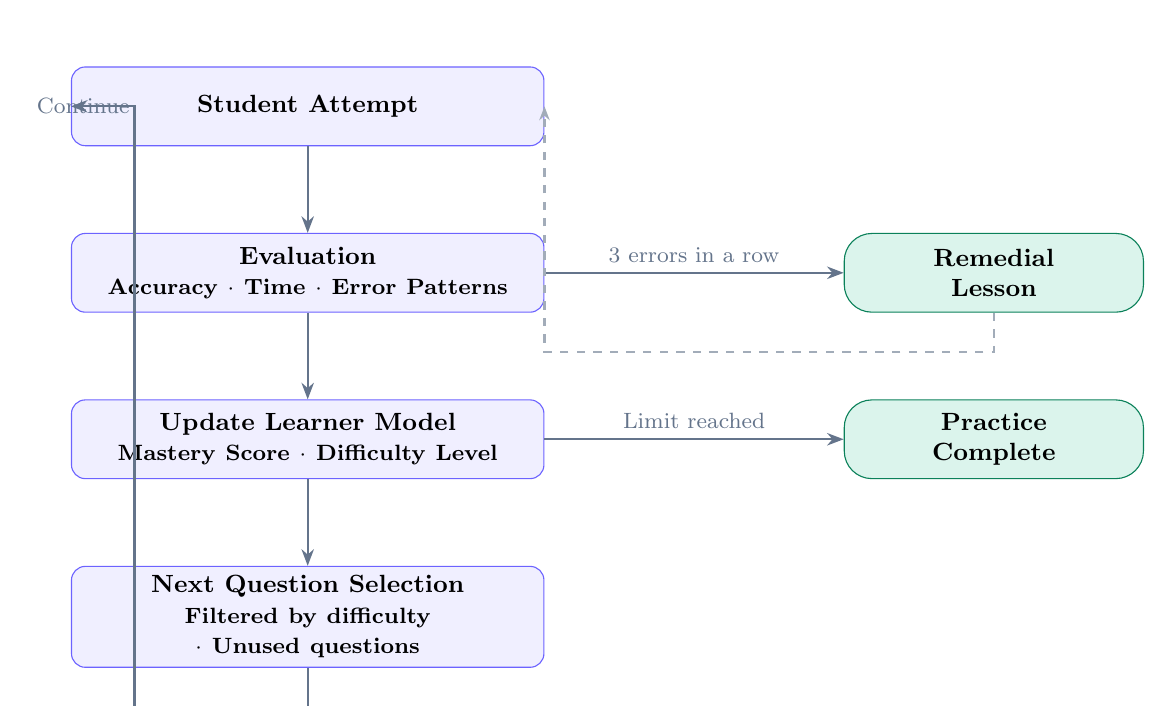
\begin{tikzpicture}[node distance=1.1cm]

  % Main loop nodes
  \node[wideblock] (attempt)  {Student Attempt};
  \node[wideblock, below=of attempt] (eval)
        {Evaluation\\ {\footnotesize Accuracy $\cdot$ Time $\cdot$ Error Patterns}};
  \node[wideblock, below=of eval] (update)
        {Update Learner Model\\ {\footnotesize Mastery Score $\cdot$ Difficulty Level}};
  \node[wideblock, below=of update] (select)
        {Next Question Selection\\ {\footnotesize Filtered by difficulty $\cdot$ Unused questions}};

  % Peripheral nodes
  \node[terminal, right=3.8cm of eval] (remedial)   {Remedial\\Lesson};
  \node[terminal, right=3.8cm of update] (complete) {Practice\\Complete};

  % Main arrows
  \draw[arrow] (attempt)  -- (eval);
  \draw[arrow] (eval)     -- (update);
  \draw[arrow] (update)   -- (select);
  \draw[arrow] (select.south) -- ++(0,-0.6) -| ++(-2.2,0) |-
               node[left, font=\footnotesize, xshift=2pt]{Continue} (attempt.west);

  % Branch: remedial
  \draw[arrow] (eval.east) -- node[above, font=\footnotesize]{3 errors in a row}
               (remedial.west);
  \draw[dasharrow] (remedial.south) -- ++(0,-0.5) -| (attempt.east);

  % Branch: complete
  \draw[arrow] (update.east) -- node[above, font=\footnotesize]{Limit reached}
               (complete.west);

\end{tikzpicture}
\captionof{figure}{The adaptive learning loop. Each attempt feeds the
evaluation engine, which updates the learner model and drives the next
question selection. Remediation and session completion are triggered by
threshold conditions.}
\end{center}

\subsection{Session Initialisation}

When a student begins a practice session for a knowledge node, the system
first \emph{classifies} the learner based on their accumulated performance
history.  This classification maps onto a target starting difficulty:

\begin{itemize}[leftmargin=1.8em]
  \item A learner classified as \textbf{struggling} (low accuracy, high error
        counts) begins at Easy difficulty.
  \item A learner classified as \textbf{average} begins at Medium difficulty —
        the default starting point.
  \item A learner classified as \textbf{advanced} (high mastery, strong recent
        performance) begins at Hard difficulty.
\end{itemize}

The first question is selected from the difficulty band appropriate to the
learner's classification, excluding any questions already seen in previous
sessions.

\subsection{During the Session: Observation and Adaptation}

After each submitted answer, the system observes three dimensions
simultaneously:

\begin{enumerate}[leftmargin=2em, itemsep=4pt]
  \item \textbf{Correctness} — was the answer right or wrong?
  \item \textbf{Time taken} — did the student respond quickly, thoughtfully,
        or after prolonged struggle?
  \item \textbf{Error type} — if the answer was wrong, which misconception
        does the selected distractor reveal?
\end{enumerate}

These observations are integrated into the learner model immediately.  The
mastery score is updated via the WMA formula (Equation~\ref{eq:wma}), the
recent performance window is extended by one entry, and any error tag is
recorded.

\subsection{Difficulty Adjustment}

The session difficulty level is re-evaluated after every question using the
recent-performance window.  Let $a$ denote the accuracy over the most recent
five responses:

\begin{equation}
  a = \frac{\text{correct answers in last 5 responses}}{5}
\end{equation}

The difficulty level $d \in \{1, 2, 3\}$ is then updated according to:

\begin{equation}
  d_{\text{new}} =
  \begin{cases}
    \min(3,\; d + 1) & \text{if } a \geq 0.80 \quad \text{(promote)} \\
    \max(1,\; d - 1) & \text{if } a < 0.50  \quad \text{(demote)} \\
    d                & \text{otherwise} \quad\quad\;\; \text{(hold)}
  \end{cases}
  \label{eq:difficulty}
\end{equation}

A change in difficulty level is communicated to the student through a
visible notification, providing transparency and motivational context
(e.g.\ ``You're on a roll — moving to harder questions'' or ``Let's
reinforce this concept before moving on'').

\subsection{Remediation}

If a student answers three consecutive questions on the same concept
incorrectly, the system interprets this as evidence that additional practice
alone is insufficient. Rather than presenting a fourth question, it delivers
a \emph{remedial lesson} — a focused re-teaching of the concept through
explanation, worked examples, and conceptual prompts.  After completing the
remedial material, the student retries the original question.

This approach is grounded in the \emph{learning by correcting errors}
literature: students benefit most from instruction that directly addresses
the specific gap revealed by their errors, delivered at the moment the gap
is detected.

\subsection{Three-Level Hint Scaffolding}

Students may request hints before submitting an answer.  The hint system
provides three levels of progressively increasing support:

\begin{description}[leftmargin=2em, style=nextline]
  \item[\textbf{Level 1 — Conceptual cue}]
    A brief reminder of the relevant principle, without revealing any steps.
    Example: ``Remember: \,`decreased by'\, is a subtraction, not addition''.

  \item[\textbf{Level 2 — Procedural guidance}]
    A step-by-step description of the solution process without giving the
    answer.  Example: ``Step 1: identify which quantity is being reduced.
    Step 2: write it first in your expression.''

  \item[\textbf{Level 3 — Worked example}]
    A parallel problem, fully solved, that the student can use as a model.
\end{description}

Each hint level used reduces the attempt score $S$ (Table~\ref{tab:scores}),
so the mastery increment for a hint-assisted correct answer is smaller than
for an unaided correct answer.  This accurately models the difference between
\emph{guided} and \emph{independent} mastery.

\subsection{Session Completion}

A practice session ends when any of the following conditions is satisfied:

\begin{itemize}[leftmargin=1.8em]
  \item The student has answered ten questions in the session (the session
        question limit), ensuring a focused and time-bounded experience;
  \item The question bank for the current concept has been exhausted —
        every available question has been presented at least once;
  \item The student chooses to end the session manually after completing the
        final available question.
\end{itemize}

% ─────────────────────────────────────────────────────────────────────────────
\section{Adaptive Question Selection}
% ─────────────────────────────────────────────────────────────────────────────

\subsection{Selection Principles}

Question selection is governed by three principles, applied in order of
priority:

\begin{enumerate}[leftmargin=2em, itemsep=4pt]
  \item \textbf{Difficulty match} — the selected question should be at the
        current adaptive difficulty level, ensuring the student operates in
        their zone of proximal development.
  \item \textbf{Novelty} — questions already answered in the current session
        are not repeated, maintaining variety and preventing rote memorisation
        of specific answers.
  \item \textbf{Availability fallback} — if the question bank at the target
        difficulty is temporarily exhausted, the system selects from
        \emph{adjacent} difficulty levels (one step easier or harder), then
        from any remaining question if necessary.
\end{enumerate}

\subsection{Fallback Strategy}

The three-stage fallback strategy ensures the session always continues as
long as unused questions remain in the bank:

\begin{center}
\begin{tabular}{cll}
  \toprule
  \textbf{Stage} & \textbf{Pool Definition} & \textbf{Activated When} \\
  \midrule
  1 & Questions at target difficulty, not yet used & First choice \\
  2 & Questions one level easier or harder, not yet used & Stage 1 is empty \\
  3 & Any remaining unused question & Stage 2 is empty \\
  \bottomrule
\end{tabular}
\captionof{table}{Fallback stages for question selection.}
\end{center}

A question is chosen uniformly at random from the winning pool so that
the student does not encounter questions in a predictable order.

% ─────────────────────────────────────────────────────────────────────────────
\section{Error Tracking and Misconception Management}
% ─────────────────────────────────────────────────────────────────────────────

\subsection{The Role of Misconceptions in Algebra Learning}

Research in mathematics education consistently identifies that algebra errors
are not random.  They arise from systematic \emph{misconceptions} — stable,
incorrect mental models that students apply consistently across problems.
Common examples include:

\begin{itemize}[leftmargin=1.8em]
  \item Treating subtraction as commutative (writing $9 - n$ instead of
        $n - 9$ because the student does not yet understand directionality);
  \item Applying a multiplier to only the first term in a bracket
        (missing the full scope of distribution);
  \item Confusing multiplication with addition (writing $7n$ as $7 + n$
        because both are sometimes described as ``combining'').
\end{itemize}

Effective tutoring requires not only detecting errors but
\emph{diagnosing their cause} — so that feedback addresses the root
misconception rather than merely marking the surface answer wrong.

\subsection{Error Tag Vocabulary}

AlgebraQuest uses a structured vocabulary of error tags to classify
misconceptions.  The vocabulary is designed to describe the \emph{cognitive
cause} of the error, not the surface form.  A representative selection:

\begin{center}
\begin{tabular}{p{4.5cm} p{7.5cm}}
  \toprule
  \textbf{Error Tag} & \textbf{Misconception Description} \\
  \midrule
  \texttt{subtraction\_reversal}    & Student reverses the order of subtraction operands \\
  \texttt{sign\_error}              & Student loses or incorrectly assigns a negative sign \\
  \texttt{missing\_bracket}         & Student applies a multiplier to only one term in a sum \\
  \texttt{coefficient\_confusion}   & Student treats a numerical coefficient as a variable \\
  \texttt{wrong\_operation}         & Student applies the wrong arithmetic operation \\
  \texttt{order\_of\_operations}    & Student performs operations in incorrect sequence \\
  \texttt{partial\_calculation}     & Student stops after the first of several required steps \\
  \texttt{bracket\_confusion}       & Student misinterprets the scope of a bracket \\
  \bottomrule
\end{tabular}
\captionof{table}{Error tag vocabulary and misconception descriptions.}
\end{center}

\subsection{Accumulation, Flagging, and Response}

Error tags are accumulated at two levels:

\begin{itemize}[leftmargin=1.8em]
  \item \textbf{Node level}: errors are recorded per knowledge concept,
        enabling concept-specific remediation.
  \item \textbf{Global level}: errors are aggregated across all concepts,
        enabling detection of cross-cutting misconceptions that appear in
        multiple contexts.
\end{itemize}

When the same error tag accumulates three or more times globally, it is
\emph{flagged} as a priority concern.  The system then:

\begin{enumerate}[leftmargin=2em]
  \item Surfaces a targeted alert identifying the misconception by name;
  \item Prioritises remedial content that specifically addresses that
        misconception category;
  \item Temporarily reduces the difficulty of subsequent questions to
        rebuild the conceptual foundation before harder problems are
        presented.
\end{enumerate}

% ─────────────────────────────────────────────────────────────────────────────
\section{Future Improvements}
% ─────────────────────────────────────────────────────────────────────────────

\subsection{Per-Concept Mastery Graphs}

The current learner dashboard represents mastery as a scalar score per node.
A future version could render time-series visualisations of $M(t)$ per
concept, enabling learners and instructors to observe learning trajectories,
identify regression patterns, and detect plateau effects that may signal the
need for a fundamentally different instructional approach.

\subsection{Item Response Theory Modelling}

The current Weighted Moving Average model treats all questions at a given
difficulty level as equivalent.  In practice, some questions within the same
difficulty band are harder than others — whether because of the specific
numbers used, the phrasing of the stem, or the subtlety of the distractors.

Replacing or augmenting the WMA with a \textbf{1-parameter Rasch model} or a
\textbf{3-parameter IRT model} would allow the system to estimate both learner
ability $\theta$ and question difficulty $b$ on a shared scale.  The
probability of a correct response would be modelled as:

\begin{equation}
  P(\text{correct} \mid \theta, b) = \frac{1}{1 + e^{-(\theta - b)}}
\end{equation}

This would enable far more principled ability estimation, better-calibrated
question selection, and eventual automatic difficulty calibration as the
question bank grows.

\subsection{Spaced Repetition}

Questions from previously mastered concepts could be re-surfaced according to
a spaced-repetition schedule (such as the SM-2 or FSRS algorithm) to combat
the forgetting curve.  A student who mastered K05 two weeks ago and has not
returned to it since would be prompted to revisit it with a brief review
session.

\subsection{Personalised Learning Paths}

Currently all learners follow the same prerequisite DAG.  A recommendation
engine could dynamically reorder available nodes based on each learner's
mastery profile and error history, prioritising those with the highest
expected learning gain or the most pedagogically urgent gaps.

\subsection{Instructor-Facing Analytics}

A class-level dashboard could aggregate anonymised learner data to surface
the most common misconceptions across an entire cohort, enabling instructors
to adjust their teaching in real time — addressing persistent errors before
they become entrenched across the class.

% ─────────────────────────────────────────────────────────────────────────────
\section*{Appendix: Key Formulae}
\addcontentsline{toc}{section}{Appendix: Key Formulae}
% ─────────────────────────────────────────────────────────────────────────────

\begin{align}
  M_{\text{new}} &= 0.7 \cdot S_{\text{recent}} + 0.3 \cdot M_{\text{current}}
                  && \text{(WMA mastery update)} \\[6pt]
  \theta_{\text{mastery}} &= 0.80
                  && \text{(mastery threshold)} \\[6pt]
  \theta_{r}     &= 0.40
                  && \text{(remedial threshold)} \\[6pt]
  a              &= \frac{\text{correct}}{|\text{recent performance window}|}
                  && \text{(sliding-window accuracy)} \\[6pt]
  d_{\text{new}} &=
    \begin{cases}
      \min(3,\; d+1) & a \geq 0.80 \\
      \max(1,\; d-1) & a < 0.50 \\
      d              & \text{otherwise}
    \end{cases}
                  && \text{(adaptive difficulty, Eq.~\ref{eq:difficulty})} \\[6pt]
  P(\text{correct}) &= \frac{1}{1 + e^{-(\theta - b)}}
                  && \text{(IRT model, proposed)}
\end{align}

\bigskip

\begin{mdframed}[linecolor=primaryblue!60, linewidth=1pt,
                 innerleftmargin=12pt, innerrightmargin=12pt,
                 innertopmargin=10pt, innerbottommargin=10pt]
  \textbf{Core Design Principle.}\quad
  Every component of AlgebraQuest is animated by the same feedback loop:
  \emph{attempt — evaluate — adapt}.  The WMA mastery model ensures
  responsiveness to recent learning; the adaptive difficulty engine keeps the
  student in their zone of proximal development; the error-tagging system
  ensures that misconceptions trigger targeted instruction rather than
  undifferentiated repetition.  Together, these mechanisms aim to replicate,
  at scale, the diagnostic sensitivity of a skilled one-to-one tutor.
\end{mdframed}

\end{document}
